%%%%%%%%%%%%%%%%%%%%%%%%%%%%%%%%%%%%%%%%%
% Beamer Presentation
% LaTeX Template
% Version 1.0 (10/11/12)
%
% This template has been downloaded from:
% http://www.LaTeXTemplates.com
%
% License:
% CC BY-NC-SA 3.0 (http://creativecommons.org/licenses/by-nc-sa/3.0/)
%
%%%%%%%%%%%%%%%%%%%%%%%%%%%%%%%%%%%%%%%%%

%----------------------------------------------------------------------------------------
%	PACKAGES AND THEMES
%----------------------------------------------------------------------------------------

\documentclass{beamer}

\mode<presentation> {
	\usetheme{Madrid}

	%\setbeamertemplate{footline} % To remove the footer line in all slides uncomment this line
	%\setbeamertemplate{footline}[page number] % To replace the footer line in all slides with a simple slide count uncomment this line
	
	%\setbeamertemplate{navigation symbols}{} % To remove the navigation symbols from the bottom of all slides uncomment this line
	
	%\addtobeamertemplate{frametitle}{}{\section{\insertframetitle}} % To add all frame title into table of contents automacitally
	
	%\setbeamertemplate{items}[square]
}

\usepackage{graphicx}
\usepackage{booktabs} % Allows the use of \toprule, \midrule and \bottomrule in tables

%----------------------------------------------------------------------------------------
%	TITLE PAGE
%----------------------------------------------------------------------------------------

\title[DragonFly]{DragonFly - Surveil Transport sector into Smart City}
%\title[Traffic Policing]{ Intelligent Policing of Traffic}
\author[Group1]{
	{\small \textit{Guided by:}} Dr. Rafeeque P.C \\
	\medskip
	{\small \textbf{\textit{Group 1}}} \\
	Abhinand C \\
	Edwin Jose George \\
	Lavanya E.V \\
	Shilpa Suresh
}
\institute[GCEK]{Government College of Engineering Kannur}
\date{\today}

\begin{document}

\begin{frame}
\titlepage
\end{frame}

\begin{frame}
\frametitle{Contents}
\tableofcontents
\end{frame}

%----------------------------------------------------------------------------------------
%	PRESENTATION SLIDES
%----------------------------------------------------------------------------------------

%------------------------------------------------
\section{Problem Statement}
\begin{frame}
	\frametitle{Problem Statement}
	%To provide a facility to track public vehicles, see their trip status and monitor their path. Also provide facility to track vehicles, detect accidents using image processing to provide safe public transport system. 
	To provide a highly integrated platform 
\end{frame}

%------------------------------------------------
\section{Motivation and Relevance}
\begin{frame}
	\frametitle{Motivation and Relevance}
	\begin{enumerate}
		\item Enable tracking of vehicles, ie, retrieving route history by typing in the description
		\item Alert Control Room, \& emergency services in case of accident
		\item Public APIs for location of public transport, and tracking system like Indian Railway NTES system
	\end{enumerate}
\end{frame}


%------------------------------------------------
\section{Proposed Framework}
\begin{frame}
	\frametitle{Proposed Framework}
	\begin{figure}
        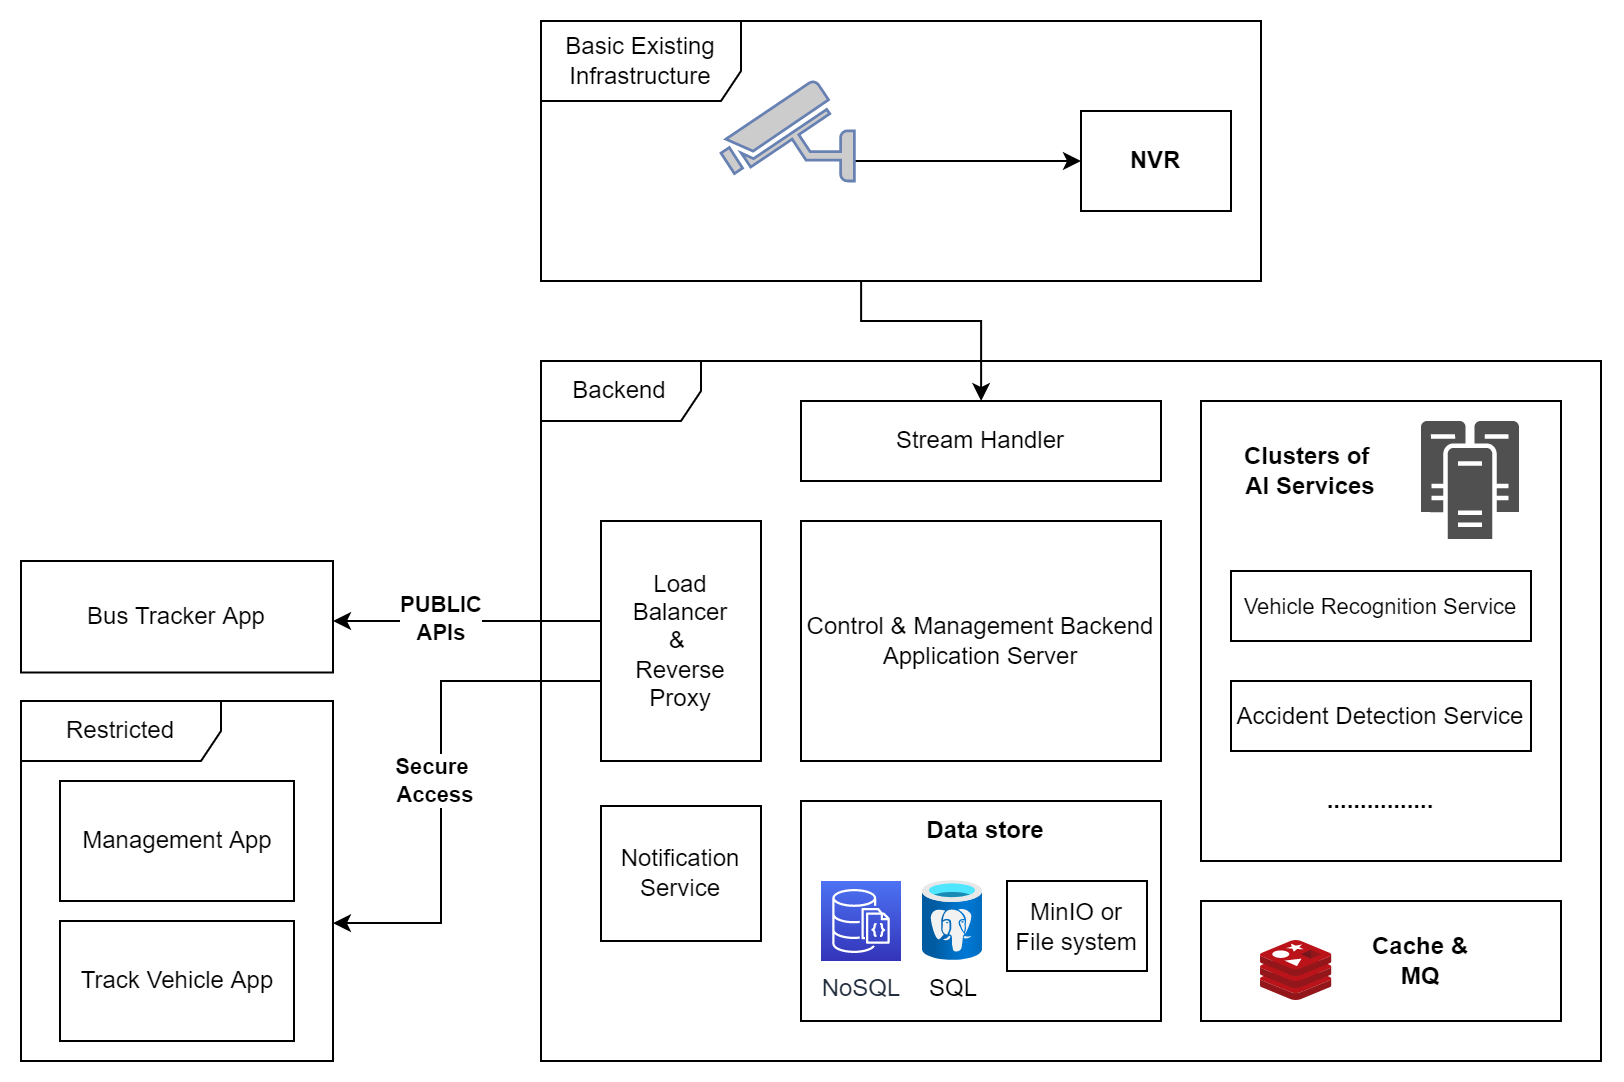
\includegraphics[width=0.8\linewidth]{res/architecture.png}
        \caption{High-level platform agnostic architecture}
    \end{figure}
\end{frame}

%------------------------------------------------
\section{Requirements}
\begin{frame}
	\frametitle{Requirements}
	content goes here...
\end{frame}


%------------------------------------------------
\section{Challenges and issues}
\begin{frame}
	\frametitle{Challenges and issues}
	content goes here...
\end{frame}


%------------------------------------------------
\begin{frame}
	\Huge{\centerline{The End}}
\end{frame}

%-------------------------incomplete infos-----------------------------
\section{Temporary info}
\begin{frame}
	The below slides are not to be included during presentation! 
\end{frame}

\subsection{Ponder points}
\begin{frame}
	\Huge{\centerline{Ponder points}}
\end{frame}

\begin{frame}
	\frametitle{What does this project do?}
	\begin{enumerate}
		\item GPS tracking of public vehicles 
		\item Predict the route and estimated time of arrival.
		\item Making use of traffic cameras to identify vehicles, track their route, helping authorities to track down a specific vehicle etc.
		\item Analysis on data to determine traffic flow to measure aspects such as speed, registration of vehicles etc to ensure regulation of traffic rules
	\end{enumerate}
\end{frame}

\begin{frame}
	\frametitle{Application Domain}
	\begin{enumerate}
		\item GPS Locating public transport buses, their schedule and route plannings
		\item Educational and other firms to track and monitor their transport system. (Q: What about GPS, it's being made mandatory)
		\item Tracking down corrupt drivers/vehicles \\(check on pollution/insurance/registration-permits, tagging specifying vehicle etc)
		\item Enforcement of traffic rules. (Speed limits, helmets for 2 wheels etc)
		\item Alerting the suggesting routes for emergency services like ambulance, fire-force etc.
		\item Accident detection
		\item Automating Surveillance footage monitoring
	\end{enumerate}
\end{frame}

\begin{frame}
	\frametitle{Features}
	\begin{enumerate}
		\item Route tracking and planning
		\item Analysing traffic using deep learning
		\begin{itemize}
		    \item Accident Alert system
		    \item Traffic rules and looking up insurance, pollution, permits etc of vehicles
		    \item Ambulance and police,.. .safety
		    \item Google like intuitive search engine for tracking specific vehicles
		\end{itemize}
		\item Public APIs for locating units. (Indian Railways)
	\end{enumerate}
\end{frame}

1. Location based AR/MR for intuitive navigation experience  
2. Natural Language based querying

\begin{frame}
	\frametitle{Limitation at sight?}
	\begin{enumerate}
		\item Real time image processing needs significant hardware support.	
		\item How to detect accidents, where to deploy hardware units?
		\item Traffic cameras can effected be from blind spots.
		\item Video capture difficulty
		\begin{itemize}
			\item Moving vehicles might give blurry image
			\item Environmental factors (rain, fog)
			\item Light beams of vehicles in night light can blind the camera
		\end{itemize}
		\item Scale up issues
		\begin{itemize}
			\item hardware processing limitation
			\item Addressing vast variety of vehicles (issue of smart cities)	
		\end{itemize}
		\item Legal considerations
		\item Privacy Policy
	\end{enumerate}
\end{frame}
%----------------------------------------------------------------------------------------

\end{document} 